% This is samplepaper.tex, a sample chapter demonstrating the
% LLNCS macro package for Springer Computer Science proceedings;
% Version 2.20 of 2017/10/04
%
\documentclass[runningheads]{llncs}
\usepackage[usenames,dvipsnames,svgnames,table]{xcolor}
\usepackage{graphicx}
\graphicspath{ {img/} }
\parindent=0
% Used for displaying a sample figure. If possible, figure files should
% be included in EPS format.
%
% If you use the hyperref package, please uncomment the following line
% to display URLs in blue roman font according to Springer's eBook style:
% \renewcommand\UrlFont{\color{blue}\rmfamily}

\begin{document}
%
\title{TRANSICIÓN A ENERGÍAS SUSTENTABLES}
%
%\titlerunning{Abbreviated paper title}
% If the paper title is too long for the running head, you can set
% an abbreviated paper title here
%
% First names are abbreviated in the running head.
% If there are more than two authors, 'et al.' is used.
\author{Dustin Mulvaney}
\institute{San José State University -
San José, CA, USA}
\maketitle
\setcounter{section}{8}
\section{INDUSTRIAS CON BAJA EMISIÓN DE CARBONO Y EL ENTORNO URBANIZADO}
\subsection{Eficiencia energética y construcciones limpias}

El entorno urbanizado requiere cantidades de energía y materiales considerables. Las industrias usan alrededor de un tercio del total de energía. Las construcciones son uno de los mayores desafíos en la descarbonización y en la transición a energías más sustentables. El uso de energía de los sistemas de aire acondicionado y calentamiento por ventilación es particularmente significante ya que representa la mitad del consumo de un edificio.

California es reconocida como uno de los estados líderes en términos de eficiencia energética. Ha dado un gran paso hacia el uso de menos energía y la mayor obtención de sus fuentes renovables. Esto es un fenómeno que en California es conocido como el efecto Rosenfeld, que sugiere un menor ratio de crecimiento en electricidad por los estándares de eficiencia energética.
\begin{center}
\textcolor{cyan}{Un \textbf{negawatt}, solía describir una cantidad de energía evitada.}\end{center}

El uso de energía para el calentamiento y enfriamiento de espacios es un área primordial en el consumo de energía en edificios y hogares. Algunas bombas de calor son de aire-aire, obteniendo calor del exterior en un día frío e ingresando en el interior. Las bombas de calor geotérmico son tierra-aire, lo que significa que obtienen aire tibio en el suelo y enviándolo al interior. Las bombas de calor también pueden calentar el agua. Estas son llamadas bombas de calor aire-agua, toman calor del exterior y lo transmiten al agua, para que puedan ser usadas en aplicaciones donde se necesite agua caliente. El ecologizar edificios tienen claros beneficios.

\textbf{El Efecto Rosenfeld\\
El uso de electricidad total per cápita se ha mantenido en una meseta en California en las últimas cuatro décadas mientras que ha aumentado a gran ritmo en el resto de Estados Unidos. Art Rosenfeld comenzó como una estrategia de costo-efectividad para ahorrar recursos energéticos y reducir los impuestos de energía de los consumidores.}

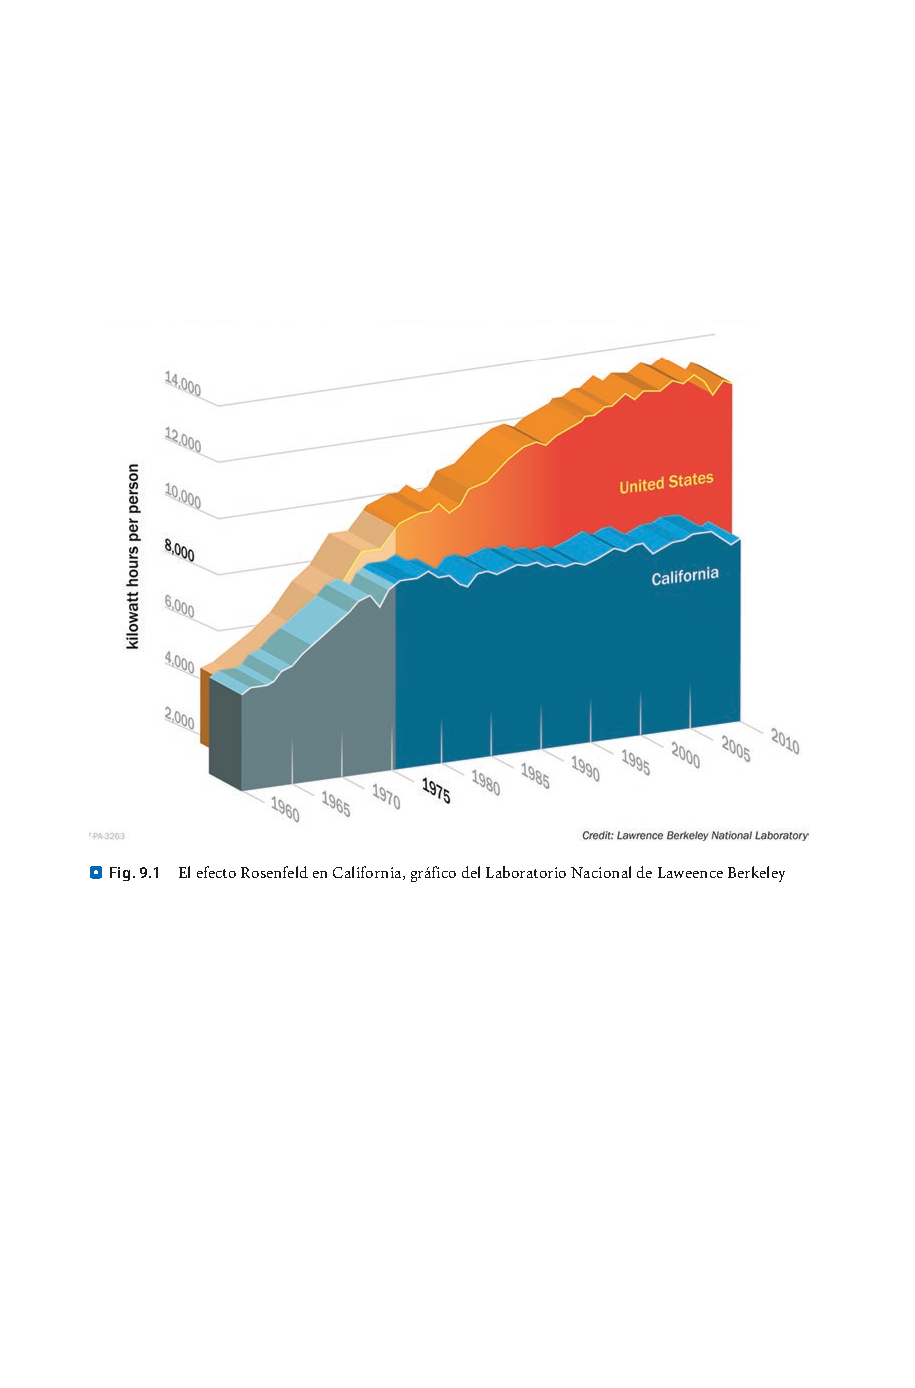
\includegraphics[scale=0.95]{9(1).pdf}

\subsection{Infraestructura para Agua y Agua Residual}
El mayor uso de energía y fuentes de GHG en cualquier municipalidad o comunidad está relacionada con el aprovisionamiento de agua potable y el desecho de aguas residuales. La energía requerida para producir agua potable depende de donde estas, que tan cerca está la fuente y la calidad de la misma. 
Las aguas residuales generan otro grupo aparte de desafíos. Podrían haber otros medios para el desecho de aguas residuales y su tratamiento. La emisión de agua residual puede contener también metano GHG. Esto es debido a que la descomposición anaeróbica de materia orgánica ocurre en sumideros, también llamada metanogénesis.
\begin{center}
\textcolor{cyan}{\textbf{Metanogénesis} es un camino metabólico donde los microorganismos digieren anaeróbicamente materiales orgánicos y producen metano.}\end{center}

\subsection{Producción de cemento}
Nos centraremos en la producción de cemento,  que es un área importante en la descarbonización de la Industria. El cemento es todo a nuestro alrededor,  es una de las sustancias más utilizadas en la Tierra. La técnica para producir cemento en horno consume mucha energía y además emite CO2  por reacción química. Cada tonelada de cemento produce alrededor de una tonelada de CO2. De hecho, las estimaciones de las emisiones globales de dióxido de carbono sitúan al cemento en alrededor del 6 \% del total. 

Un ejemplo de la producción de CO2 es:
\begin{center}
\includegraphics{formula.pdf}\end{center}
Un cambio que podríamos hacer para reducir las emisiones es cambiar el combustible por un combustible menos intensivo en carbono. 

Para mejorar la eficiencia energética de la producción de cemento se busca generar un cambio tecnológico, podría ser un cambio tecnológico en el tipo de hornos. La producción del cemento Portland  está llegando a su capacidad límite  para ser más eficientes.Otra cosa que se podría hacer es la sustitución de materiales, debemos sustituir los sulfoaluminato de calcio y los silicatos de calcio. 
 
Varias empresas cementeras están tratando de mejorar en las emisiones de carbono, pero como el precio del carbono no baja, se les hace difícil invertir en las emisiones. 
Además, se prevé que el crecimiento del cemento siga aumentando en las próximas décadas. Por lo tanto es de vital importancia producir con menos emisiones a medida que avanzamos.
Este cambio puede llevar mucho tiempo. 

\subsection{Mejores Aleaciones y Metales: Acero, Cobre, Aluminio}
La industria minera y actividades afines contribuyen en gran medida en los problemas medioambientales, como el efecto invernadero y las emisiones. El hierro y el acero generan más del 5 \% de las emisiones de efecto invernadero totales. Una tonelada de acero produce entre 1.6 a 3.1 toneladas de dióxido de carbono. Hay algunos de los procesos fundamentales que no pueden cambiar, aunque cada vez hay más operaciones de minería y fundición (principalmente en Europa del Norte) que se están haciendo con electricidad renovable, como la eólica y la hidroeléctrica. Por lo tanto, estos impactos energéticos son el producto “paisajes energéticos” sobre los que se constituyen.

Se requiere una investigación de la economía circular de los principales metales y aleaciones. Se puede reducir en gran medida la huella medioambiental que dejan los materiales reciclados de metales al ser utilizados en los productos. Al cerrar este círculo se obtienen una baja en el consumo de energía y emisión de gases de efecto invernadero, comparado con los metales vírgenes (acero, cobre, aluminio).Además, la recuperación de los metales semiconductores reducen la carga medioambiental de los materiales fotovoltaicos. Si se combinan diferentes tipos de de metales, el reciclado se vuelve más complejo, cuando históricamente eran materiales homogéneos. Por ejemplo, se dificulta el reciclaje de acero debido a la contaminación con cobre proveniente de los compuestos eléctricos de los autos Los compuestos plásticos, a su vez, complican la situación. El aluminio reciclado puede reducir el consumo de energía diez veces en comparación a hacerlo desde la Bauxita.

Hay compañías que están experimentando juntar o concentrar los metales buscados con ayuda de organismos biológicos. Una bio mina es la que recolecta desechos electrónicos de otros residuos que contienen metales y permite la recuperación de los productos desechados.

En lugares donde hay un rápido crecimiento de la economía global, la cual requiere nuevos metales para nuevas tecnologías, no es suficiente buscar una segunda vida del metal. Se pueden requerir actividades de minería. Los progresos en la recolección de metales de agua salada son una opción viable, especialmente si se vinculan con plantas desalinizadoras. Hay otras propuestas para recolección de metales de salmueras geotermales o de la extracción de petróleo y gas. Un área de investigación sobre la descarbonización a corto plazo será la electrificación y el uso de hidrógeno en la industria.

\subsection{Industrias Químicas}
La industria química es un área en la que se debe actuar para avanzar hacia la descarbonización ya que es la responsable del 10 porciento de las emisiones globales de gases de efecto invernadero. Del total de la energía consumida por la industria, dos tercios corresponden a aquellas que usan calor a altas temperaturas como los fabricantes de plásticos y amoníaco, además muchas utilizan el vapor para calefaccionar reactores y otras tareas. La electrificación de estos y otros procesos puede contribuir a reducir las emisiones, o también se puede utilizar el amoníaco como combustible ya sea directamente o bien crackeado por su contenido de hidrógeno (la combustión del amoníaco da como productos nitrógeno gaseoso y vapor de agua, evitando la producción de CO2).

La industria química está interconectada con compañías energéticas. Por un lado, muchas de las materias primas de la industria química son compradas a la industria del petróleo, como es el caso del etano que se utiliza para la fabricación de plásticos, por otro lado, la industria química es una importante proveedora de materiales para la industria fotovoltaica.

Los principios de la química verde se encuentran liderando la sustentabilidad de este sector, además de que algunas se encuentran involucradas activamente con la responsabilidad social empresaria. Hoy en día, gran parte del esfuerzo consiste en garantizar que los materiales nocivos sean eliminados de los plásticos, como es el caso de los halógenos o retardantes de llama bromados. Un siguiente paso deberá hacer foco en la degradación de los plásticos, para resolver los problemas de contaminación plástica y climática simultáneamente.

Será necesario realizar descubrimientos en el área de los bioplásticos, que permitan reemplazar a los realizados a partir del gas natural o etano. Aún hay muchas dudas sobre la calidad y durabilidad de los bioplásticos, por lo que aún serán difíciles de implementar. Pero cualquier avance lejos de los plásticos provenientes de combustibles fósiles ayudará con los problemas de plásticos en el mediambiente.

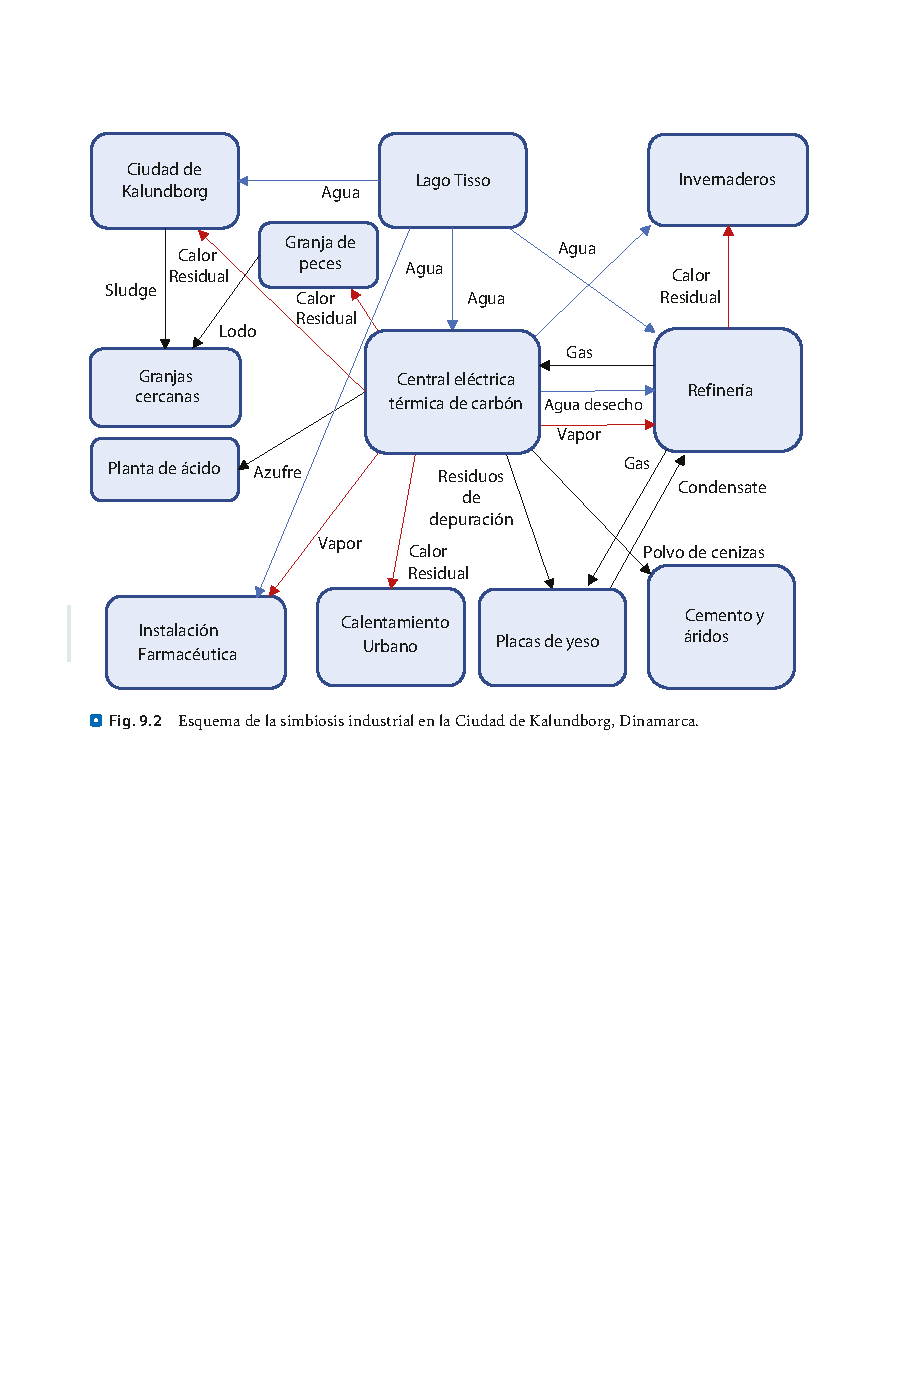
\includegraphics[scale=0.95]{9(2).pdf}

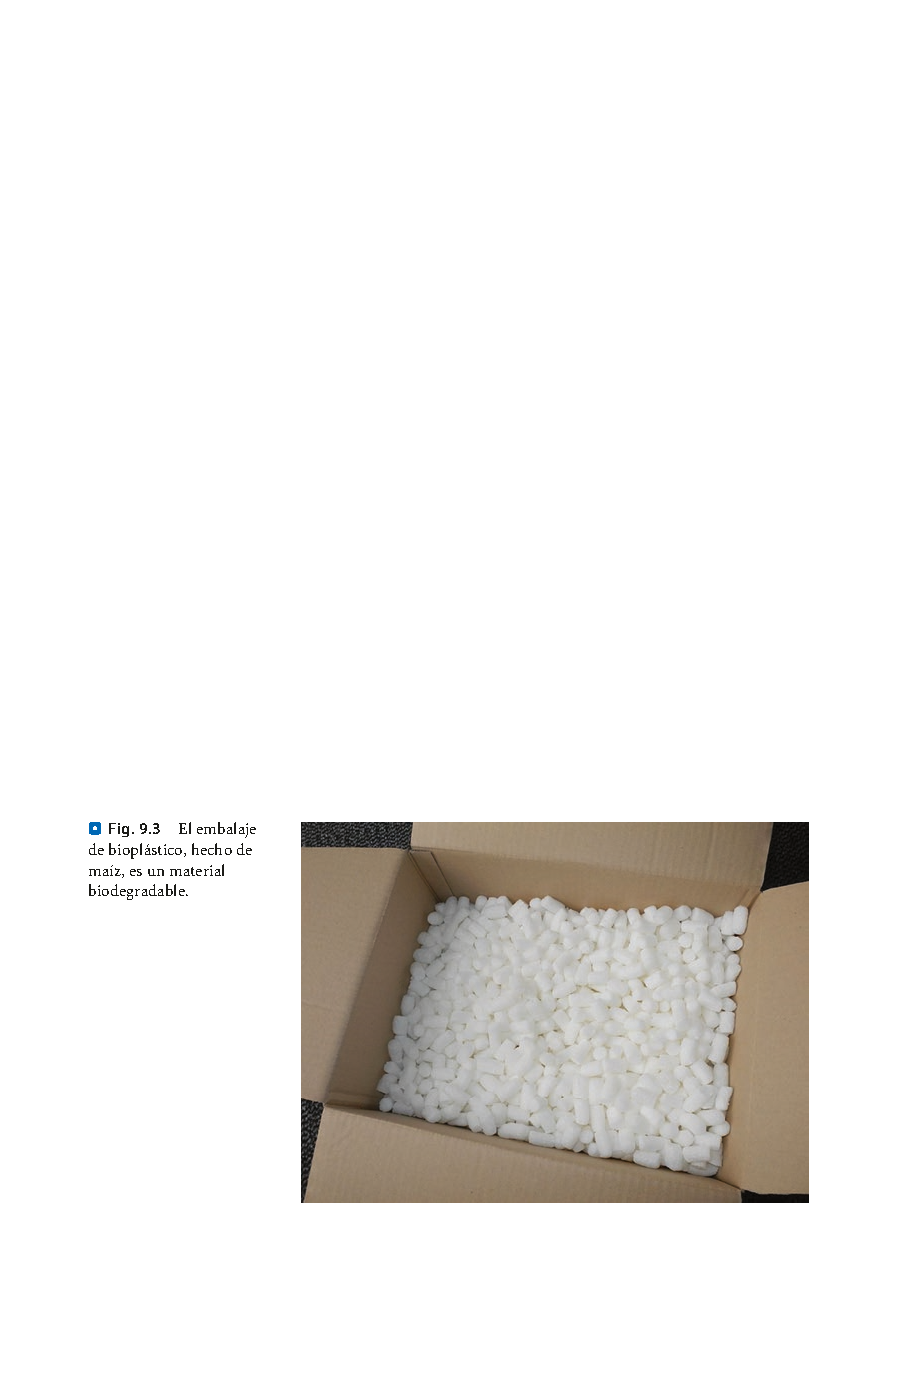
\includegraphics[scale=0.95]{9(3).pdf}

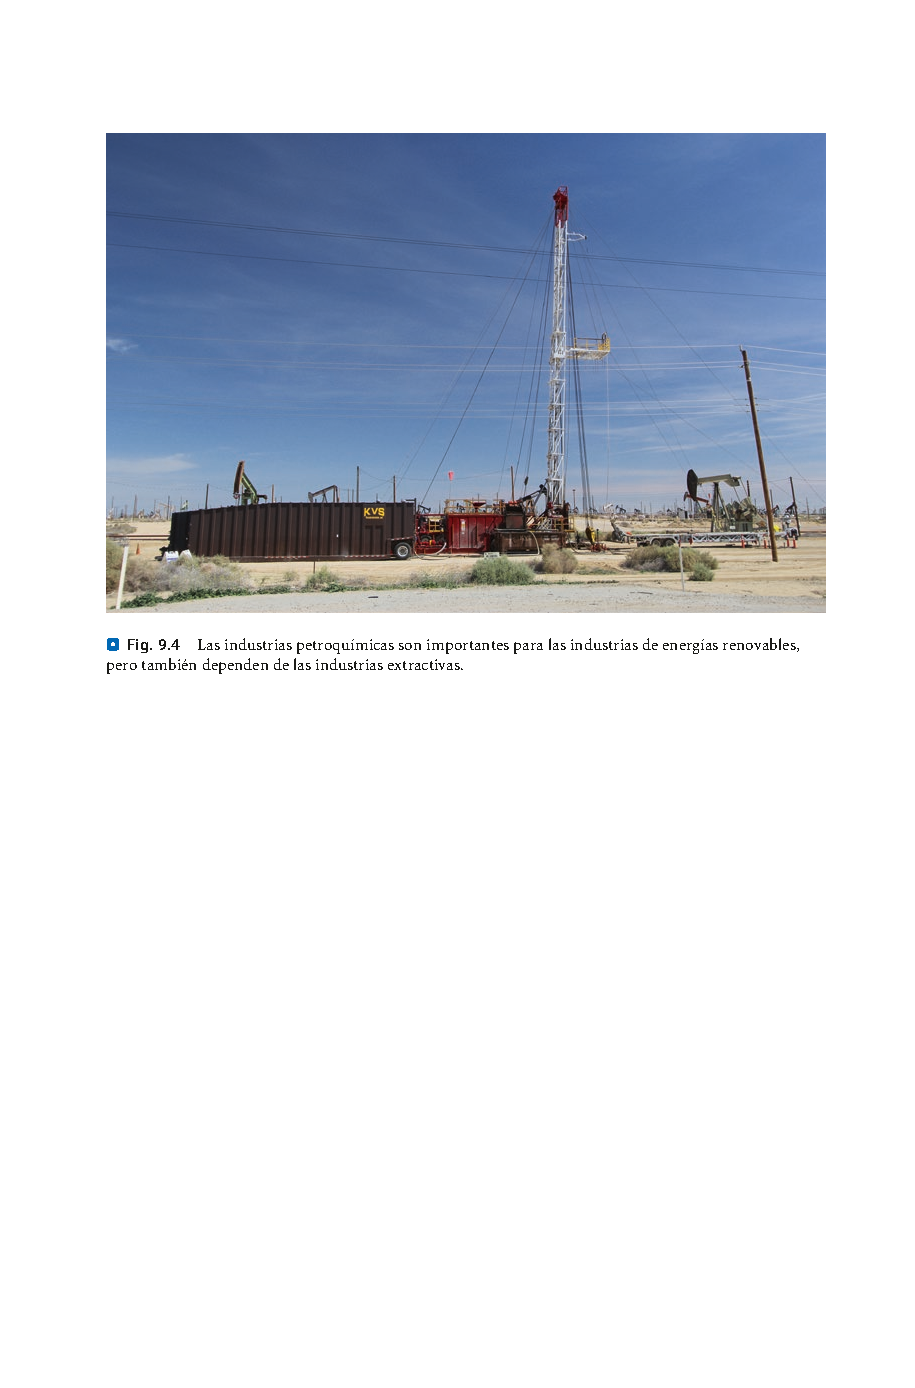
\includegraphics[scale=0.95]{9(4).pdf}

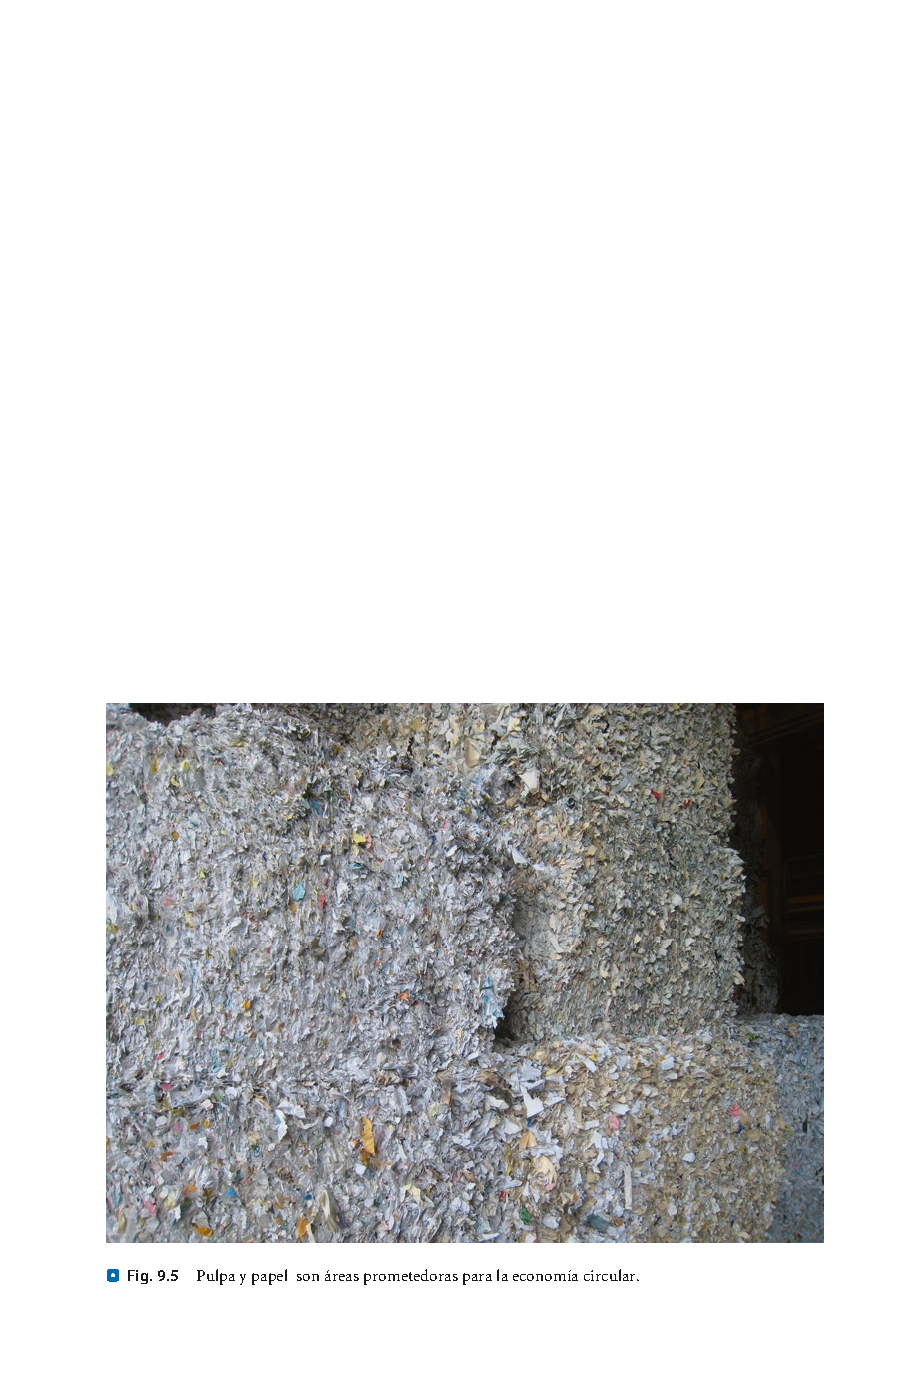
\includegraphics[scale=0.95]{9(5).pdf}


\subsection{REVISION}
Guido Scopel,Legajo 11766

% the environments 'definition', 'lemma', 'proposition', 'corollary',
% 'remark', and 'example' are defined in the LLNCS documentclass as well.
%

%
% ---- Bibliography ----
%
% BibTeX users should specify bibliography style 'splncs04'.
% References will then be sorted and formatted in the correct style.
%
% \bibliographystyle{splncs04}
% \bibliography{mybibliography}
%


\end{document}
